JavaScript is well supported in virtually all web browsers on both desktop and mobile \parencite{Zakai2011}. According to \textcite{TiwariSolihin2012} more than 95\% of all web pages are viewed with JavaScript enabled web browsers and more than 99\% of all web sites use JavaScript. However, while web apps have an advantage of portability compared to native mobile apps, the dynamic typing and prototypes features of JavaScript makes it execution inefficient \parencite{ParkJungMoon2015}. \textcite{HaasRossbergSchuffTitzerHolmanGohmanWagnerZakaiBastien2017} notes that while the web has given rise to demanding web apps, JavaScript as a language being the only programming language available in web browsers, is not very well equipped to support such applications. \textcite{ReiserBlaser2017} describe that there is always a desire for higher performance in web applications and \textcite{Zakai2018} describe JavaScript as an obstacle for demanding high-performing apps. The last few years manufacturers of web browsers has been focused on optimizing JavaScript performance through just-in-time (JIT) and ahead-of-time (AOT) compilation \parencite{HerreraChenLavoieHendren2018}.

\begin{figure}[!h]
\centering
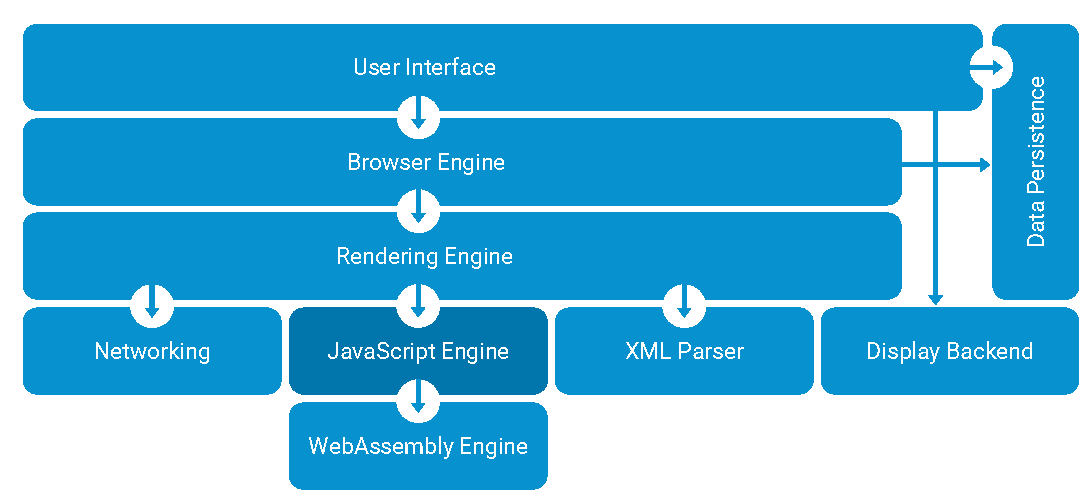
\includegraphics[width=16cm,keepaspectratio]{../Figures/reference-architecture}
\caption{Web browser reference architecture. Adapted from \textcite{GrosskurthGodfrey2005}.}
\label{reference-architecture}
\end{figure}

The component in a web browser that is focused on JavaScript interpretation and execution is called a JavaScript engine \parencite{JeonChoi2012} The JavaScript engine is illustrated in Figure \ref{reference-architecture} as a part of the web browser reference architecture developed by \textcite{GrosskurthGodfrey2005}. The way JavaScript is executed is somewhat different in different web browsers but all share a similar approach. Figure \ref{javascript-optimization} illustrates three tiers of executing JavaScript. The first tier is concerned with interpreting the source code in realtime, translating that into an Abstract Syntax Tree (AST) and use that to generate bytecode that is then executed. Before browser vendors saw a competitive in having a really fast JavaScript engine the first tier was the only job of the JavaScript engine. In the second and third tier the result of the compilation is stored and executed again, the JIT compilation and the optimized JIT compilation is invoked based on how ''hot'' the code is \parencite{KedlayaRobatmiliHardekopf2015,ParkKimParkMoon2018}.

\begin{figure}[!h]
\centering

\includegraphics[width=16cm,keepaspectratio]{../Figures/javascript-optimization}
\caption{JavaScript execution tiers. Adapted from \textcite{ParkKimMoon2017,ZhuykovVardanyanMelnikBuchatskiySharygin2015}.}
\label{javascript-optimization}
\end{figure}        

As another way to try to optimize JavaScript \textcite{ParkJungMoon2015,ZhuykovVardanyanMelnikBuchatskiySharygin2015} and others are currently experimenting with AOT compilation where JavaScript is actually compiled ahead of time instead of in realtime.

\subsubsection{TypeScript}

JavaScript does not have a static type system \parencite{Park2014}. TypeScript is a superset of JavaScript that adds type information \parencite{DeWolffHage2017}. Type information allows the programmer to see mistakes sooner during the development phase rather than later in runtime. In Listing \ref{listing:typescript} the JavaScript function \texttt{isPrime} has been enhanced with type information.

\lstinputlisting[label=listing:typescript,language=JavaScript,caption=prime.ts]{../Listings/isprime.ts}

Before TypeScript is published as part of a web site it is transformed to regular JavaScript using the TypeScript compiler \parencite{ReiserBlaser2017}. This does thus not directly solve the problem of performance, but decreases the number of runtime errors, and enables future backend optimizations such as improved guesses by the JIT-compiler.

\subsubsection{asm.js}

Another approach to optimize JavaScript is asm.js which is a subset of JavaScript focused on performance \parencite{Zakai2018}. If the browser understands asm.js it will skip certain steps in the JavaScript engine designed to optimize ''normal'' JavaScript, as it knows that asm.js is already optimized in certain ways. \textcite{Zakai2018} describes the idea behind asm.js as removing the dynamic and complex parts of JavaScript and thus ending up with a subset that is more easily optimized by the JavaScript engines.

\lstinputlisting[label=asmjs,language=JavaScript,caption=asm.js]{../Listings/asm.js}

Listing \ref{asmjs} shows an implementation of a string calculation length function written in asm.js containing two prominent differences between asm.js and regular JavaScript. On line 2, 6, and 8 a bitwise operator \texttt{|0} is used. The operator has no effect on the value of the result but provides a hint to the JavaScript engine that the result is of the type signed integer which is information that can be used by the JavaScript engine to optimize the performance \parencite{Zakai2018}. The use of \texttt{MEM8[]} on line 5 is another way to increase the performance in asm.js. In asm.js much of the memory is written to and read from a type buffer instead of relying on the slower garbage collector provided by the JavaScript engine \parencite{Zakai2011}.

Asm.js is not meant to be written by hand but rather serve as compilation target \parencite{VanEsNicolayStievenartDHondtDeRoover2016}. The tool Emscripten \parencite{Zakai2011} was so that source code written in languages such as C/C++ could be compiled to asm.js. As asm.js is a subset of JavaScript all browsers that can run JavaScript can run asm.js code that has been created by the Emscripten tool \parencite{HaasRossbergSchuffTitzerHolmanGohmanWagnerZakaiBastien2017}. Given this, it is not far fetched to call asm.js the assembly language of the web. However, asm.js \emph{is} JavaScript and JavaScript was never designed as a compilation target \parencite{Watt2018}.
